A mesh network can use a wide variety of protocols, to manage the route data is transferred.
In networking a protocol is a special set of rules and standards for how devices would interacts with each other.
A well known protocols would be TCP/IP(Transmission Control Protocol/Internet Protocol), which today are used to communicate between anything with a internet connection.
The mesh network we are looking at is a radio based network, and therefore some more relevant protocols will be examined. 
Few excising protocols will be presented in this section.

\subsection{Time division multiple access}
Time division multiple access(TDMA) is protocol that divides a single channel into smaller time slots. Each time slot transmits one byte or a segment of a signal, in a sequential serial data format.

TDMA is as an example used in the T1 telecommunication transmission system.
Each T1 channels carry up to 24 voice telephone connections.
Where each connection covers 300 Hz to 3000Hz and is digitized at an 8-kHz rate, which is two times the highest frequency component needed to retain all the analog content.
\begin{figure}[!h]
	\centering
	\makebox[\textwidth][c]{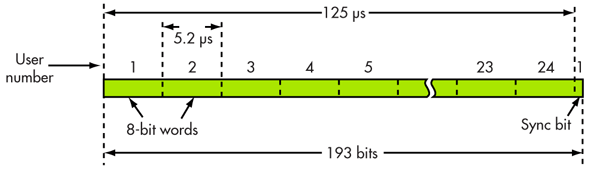
\includegraphics[width=1\textwidth]{figures/TDMA.png}}
	\caption{Illustration of the TDMA protocol}
	\label{fig:TDMAfigure}
\end{figure}

On \figref{TDMAfigure} it is seen how the channel is split up into 24 smaller pieces.
Each time slot is accountant for (in this case) a user using a voice channel.
Each time slot is of the size 8-bit, the user is unaware of this small data size, because the shift between each time slot happens so fast.
This gives the illusion of each user talking with no interruptions, even though each is assigned 1/24 of the total bandwidth.
A single bit is used to synchronization.
The TDMA system can maximum achieved a data rate of 1.544 Mbit/second.\cite{TDMA}

TDMA can be used for any system that require several device to use the same channel, whiteout interfering with each other.

\subsection{Ad hoc On-Demand Distance Vector Routing}



\subsection{Radio Link Protocol}
Radio Link protocol(RLP) is a automatic repeat request(ARQ)\footnote{An error-control method for data transmission that uses acknowledgments and timeouts} fragmentation protocol used over a wireless air interface.
Most air interface protocols have a packet loss of up to 1\% which is intolerable when handling sensitive data.
RLP detects losses in packets and with a retransmission tries to bring down the losses.
The retransmission can bring the loss down to 0.1\% to 0.0001\%.
This loss rate is more tolerable when handling sensitive and precise data.

RPL cannot request a certain payload size from the air interface, the air interface scheduler instead determines the packet size, based on changing channel conditions constantly.
Most of the other fragmentation protocols, such as 802.11b\footnote{An wireless networking specification that extends throughput up to 11 Mbit/s} and IP, determine a payload of a certain size by the upper layers, and call upon the MAC.
These protocols are not as flexible as RLP, and sometime fail transition during small fades in a wireless environment. 